\section{Thesis RESPONdING}

\begin{frame}{RESPONdING}
    \begin{center}
        Knowledge Graph-based System for Technical Document Retrieval\\A deductive reasoning-focused exploration
    \end{center}
    
    \begin{itemize}
        \item Research objective: Leveraging domain knowledge to enhance Information Retrieval in a technical context.
        \item Technical content is implicitly structured by domain knowledge.
        \item This knowledge must be explicitly machine readable.
        \item KGs are machine readable structured knowledge artifacts.
    \end{itemize}
    
    \begin{center}
        From a keyword-based search to a concept-based one.
    \end{center}
    
\end{frame}

\begin{frame}{Contributions}

    \begin{center}
        A top-down approach from a system perspective down to solution implementations.
    \end{center}

    Contributions:
    \begin{itemize}
        \item A unifying definition of Knowledge Graph
        \item An architecture for Knowledge Graph-Based Systems
        \item A framework for Ontology Learning
        \item An OWL Information Retrieval ontology
        \item A study of a text-based compared to a Knowledge Graph-based Information Retrieval system
    \end{itemize}
    
\end{frame}

\begin{frame}{Manuscript overview}
    \begin{figure} [H]
        \begin{center}
            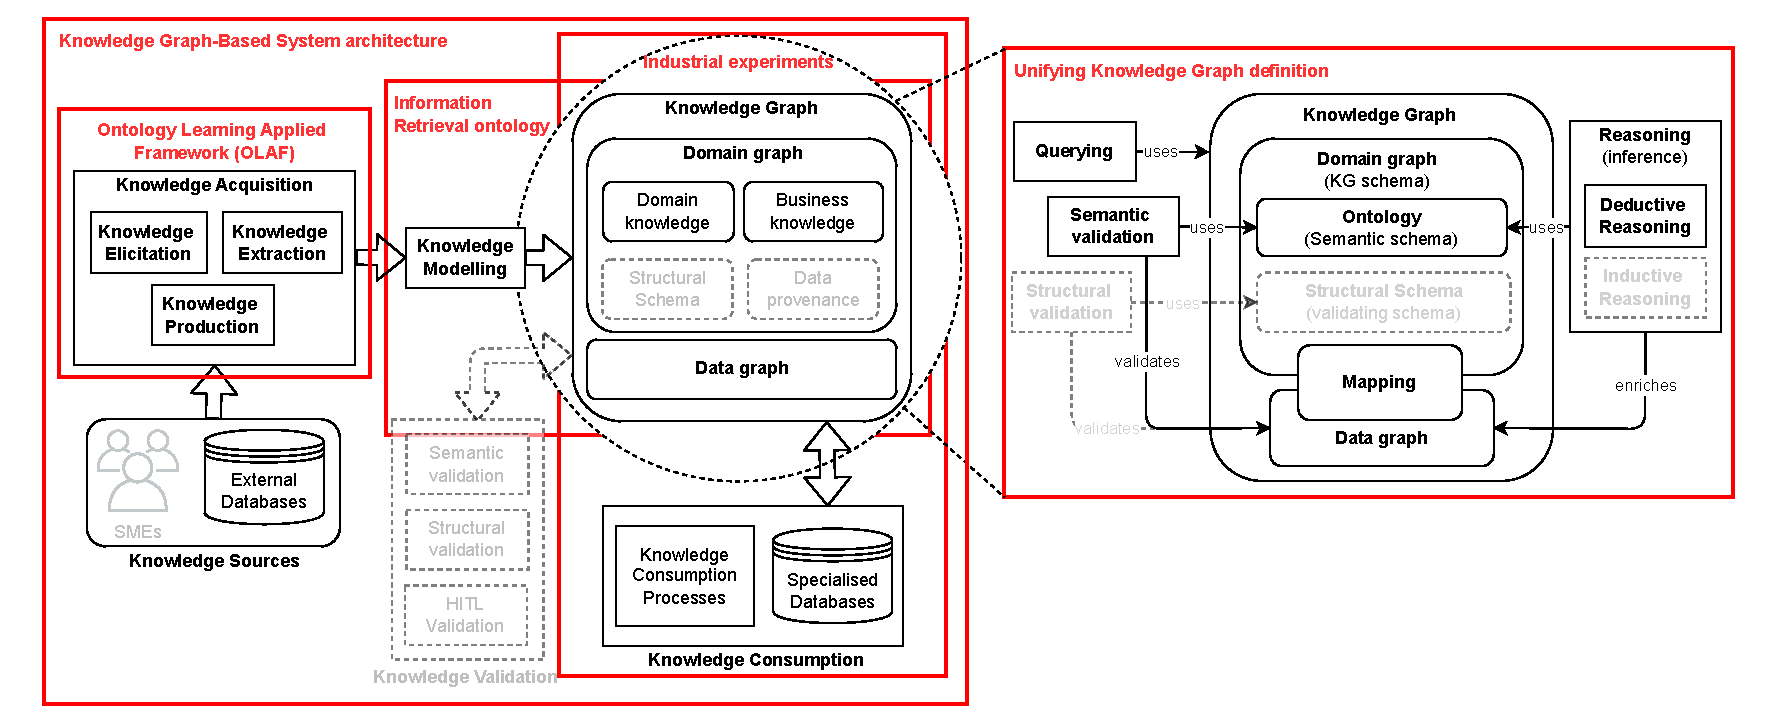
\includegraphics[scale=0.4]{images/KGBS-detailed-technos-KG-def-conclusion-simplified.pdf} 
            \caption{Manuscript overview} 
        \end{center}
    \end{figure}
\end{frame}

\begin{frame}{Knowledge Graph vs Ontology}

    \begin{figure} [H]
        \begin{center}
            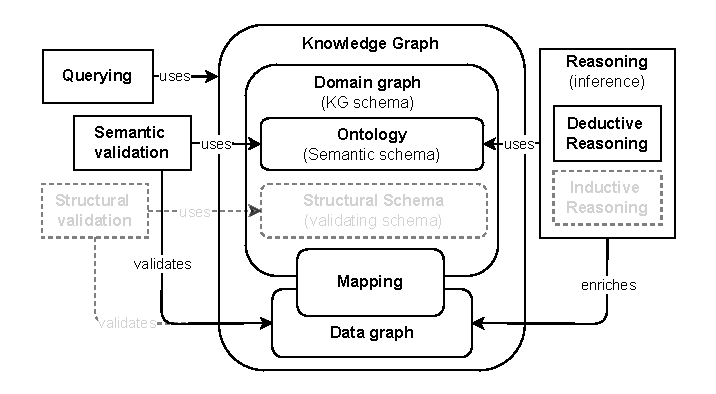
\includegraphics[scale=0.8]{images/kg-def-simple.pdf} 
            \caption{Knowledge Graph definition} 
        \end{center}
    \end{figure}

\end{frame}

% \begin{frame}{Table of contents ?}

% \end{frame}